
%% bare_conf.tex
%% V1.3
%% 2007/01/11
%% by Michael Shell
%% See:
%% http://www.michaelshell.org/
%% for current contact information.
%%
%% This is a skeleton file demonstrating the use of IEEEtran.cls
%% (requires IEEEtran.cls version 1.7 or later) with an IEEE conference paper.
%%
%% Support sites:
%% http://www.michaelshell.org/tex/ieeetran/
%% http://www.ctan.org/tex-archive/macros/latex/contrib/IEEEtran/
%% and
%% http://www.ieee.org/

%%*************************************************************************
%% Legal Notice:
%% This code is offered as-is without any warranty either expressed or
%% implied; without even the implied warranty of MERCHANTABILITY or
%% FITNESS FOR A PARTICULAR PURPOSE! 
%% User assumes all risk.
%% In no event shall IEEE or any contributor to this code be liable for
%% any damages or losses, including, but not limited to, incidental,
%% consequential, or any other damages, resulting from the use or misuse
%% of any information contained here.
%%
%% All comments are the opinions of their respective authors and are not
%% necessarily endorsed by the IEEE.
%%
%% This work is distributed under the LaTeX Project Public License (LPPL)
%% ( http://www.latex-project.org/ ) version 1.3, and may be freely used,
%% distributed and modified. A copy of the LPPL, version 1.3, is included
%% in the base LaTeX documentation of all distributions of LaTeX released
%% 2003/12/01 or later.
%% Retain all contribution notices and credits.
%% ** Modified files should be clearly indicated as such, including  **
%% ** renaming them and changing author support contact information. **
%%
%% File list of work: IEEEtran.cls, IEEEtran_HOWTO.pdf, bare_adv.tex,
%%                    bare_conf.tex, bare_jrnl.tex, bare_jrnl_compsoc.tex
%%*************************************************************************

% *** Authors should verify (and, if needed, correct) their LaTeX system  ***
% *** with the testflow diagnostic prior to trusting their LaTeX platform ***
% *** with production work. IEEE's font choices can trigger bugs that do  ***
% *** not appear when using other class files.                            ***
% The testflow support page is at:
% http://www.michaelshell.org/tex/testflow/



% Note that the a4paper option is mainly intended so that authors in
% countries using A4 can easily print to A4 and see how their papers will
% look in print - the typesetting of the document will not typically be
% affected with changes in paper size (but the bottom and side margins will).
% Use the testflow package mentioned above to verify correct handling of
% both paper sizes by the user's LaTeX system.
%
% Also note that the "draftcls" or "draftclsnofoot", not "draft", option
% should be used if it is desired that the figures are to be displayed in
% draft mode.
%
\documentclass[conference]{IEEEtran}
%%\documentclass{article}
% Add the compsoc option for Computer Society conferences.
%
% If IEEEtran.cls has not been installed into the LaTeX system files,
% manually specify the path to it like:
% \documentclass[conference]{../sty/IEEEtran}

% Some very useful LaTeX packages include:
% (uncomment the ones you want to load)


% *** MISC UTILITY PACKAGES ***
%
%\usepackage{ifpdf}
% Heiko Oberdiek's ifpdf.sty is very useful if you need conditional
% compilation based on whether the output is pdf or dvi.
% usage:
% \ifpdf
%   % pdf code
% \else
%   % dvi code
% \fi
% The latest version of ifpdf.sty can be obtained from:
% http://www.ctan.org/tex-archive/macros/latex/contrib/oberdiek/
% Also, note that IEEEtran.cls V1.7 and later provides a builtin
% \ifCLASSINFOpdf conditional that works the same way.
% When switching from latex to pdflatex and vice-versa, the compiler may
% have to be run twice to clear warning/error messages.






% *** CITATION PACKAGES ***
%
\usepackage{cite}
% cite.sty was written by Donald Arseneau
% V1.6 and later of IEEEtran pre-defines the format of the cite.sty package
% \cite{} output to follow that of IEEE. Loading the cite package will
% result in citation numbers being automatically sorted and properly
% "compressed/ranged". e.g., [1], [9], [2], [7], [5], [6] without using
% cite.sty will become [1], [2], [5]--[7], [9] using cite.sty. cite.sty's
% \cite will automatically add leading space, if needed. Use cite.sty's
% noadjust option (cite.sty V3.8 and later) if you want to turn this off.
% cite.sty is already installed on most LaTeX systems. Be sure and use
% version 4.0 (2003-05-27) and later if using hyperref.sty. cite.sty does
% not currently provide for hyperlinked citations.
% The latest version can be obtained at:
% http://www.ctan.org/tex-archive/macros/latex/contrib/cite/
% The documentation is contained in the cite.sty file itself.



% *** GRAPHICS RELATED PACKAGES ***
%
\ifCLASSINFOpdf
  \usepackage[pdftex]{graphicx}
  % declare the path(s) where your graphic files are
  % \graphicspath{{../pdf/}{../jpeg/}}
  % and their extensions so you won't have to specify these with
  % every instance of \includegraphics
  % \DeclareGraphicsExtensions{.pdf,.jpeg,.png}
\else
  % or other class option (dvipsone, dvipdf, if not using dvips). graphicx
  % will default to the driver specified in the system graphics.cfg if no
  % driver is specified.
  \usepackage[dvips]{graphicx}
  % declare the path(s) where your graphic files are
  % \graphicspath{{../eps/}}
  % and their extensions so you won't have to specify these with
  % every instance of \includegraphics
  % \DeclareGraphicsExtensions{.eps}
\fi
% graphicx was written by David Carlisle and Sebastian Rahtz. It is
% required if you want graphics, photos, etc. graphicx.sty is already
% installed on most LaTeX systems. The latest version and documentation can
% be obtained at: 
% http://www.ctan.org/tex-archive/macros/latex/required/graphics/
% Another good source of documentation is "Using Imported Graphics in
% LaTeX2e" by Keith Reckdahl which can be found as epslatex.ps or
% epslatex.pdf at: http://www.ctan.org/tex-archive/info/
%
% latex, and pdflatex in dvi mode, support graphics in encapsulated
% postscript (.eps) format. pdflatex in pdf mode supports graphics
% in .pdf, .jpeg, .png and .mps (metapost) formats. Users should ensure
% that all non-photo figures use a vector format (.eps, .pdf, .mps) and
% not a bitmapped formats (.jpeg, .png). IEEE frowns on bitmapped formats
% which can result in "jaggedy"/blurry rendering of lines and letters as
% well as large increases in file sizes.
%
% You can find documentation about the pdfTeX application at:
% http://www.tug.org/applications/pdftex





% *** MATH PACKAGES ***
%
\usepackage[cmex10]{amsmath}
% A popular package from the American Mathematical Society that provides
% many useful and powerful commands for dealing with mathematics. If using
% it, be sure to load this package with the cmex10 option to ensure that
% only type 1 fonts will utilized at all point sizes. Without this option,
% it is possible that some math symbols, particularly those within
% footnotes, will be rendered in bitmap form which will result in a
% document that can not be IEEE Xplore compliant!
%
% Also, note that the amsmath package sets \interdisplaylinepenalty to 10000
% thus preventing page breaks from occurring within multiline equations. Use:
%\interdisplaylinepenalty=2500
% after loading amsmath to restore such page breaks as IEEEtran.cls normally
% does. amsmath.sty is already installed on most LaTeX systems. The latest
% version and documentation can be obtained at:
% http://www.ctan.org/tex-archive/macros/latex/required/amslatex/math/





% *** SPECIALIZED LIST PACKAGES ***
%
\usepackage{algorithm,algorithmic}
% algorithmic.sty was written by Peter Williams and Rogerio Brito.
% This package provides an algorithmic environment fo describing algorithms.
% You can use the algorithmic environment in-text or within a figure
% environment to provide for a floating algorithm. Do NOT use the algorithm
% floating environment provided by algorithm.sty (by the same authors) or
% algorithm2e.sty (by Christophe Fiorio) as IEEE does not use dedicated
% algorithm float types and packages that provide these will not provide
% correct IEEE style captions. The latest version and documentation of
% algorithmic.sty can be obtained at:
% http://www.ctan.org/tex-archive/macros/latex/contrib/algorithms/
% There is also a support site at:
% http://algorithms.berlios.de/index.html
% Also of interest may be the (relatively newer and more customizable)
% algorithmicx.sty package by Szasz Janos:
% http://www.ctan.org/tex-archive/macros/latex/contrib/algorithmicx/




% *** ALIGNMENT PACKAGES ***
%
%\usepackage{array}
% Frank Mittelbach's and David Carlisle's array.sty patches and improves
% the standard LaTeX2e array and tabular environments to provide better
% appearance and additional user controls. As the default LaTeX2e table
% generation code is lacking to the point of almost being broken with
% respect to the quality of the end results, all users are strongly
% advised to use an enhanced (at the very least that provided by array.sty)
% set of table tools. array.sty is already installed on most systems. The
% latest version and documentation can be obtained at:
% http://www.ctan.org/tex-archive/macros/latex/required/tools/


%\usepackage{mdwmath}
%\usepackage{mdwtab}
% Also highly recommended is Mark Wooding's extremely powerful MDW tools,
% especially mdwmath.sty and mdwtab.sty which are used to format equations
% and tables, respectively. The MDWtools set is already installed on most
% LaTeX systems. The lastest version and documentation is available at:
% http://www.ctan.org/tex-archive/macros/latex/contrib/mdwtools/


% IEEEtran contains the IEEEeqnarray family of commands that can be used to
% generate multiline equations as well as matrices, tables, etc., of high
% quality.


%\usepackage{eqparbox}
% Also of notable interest is Scott Pakin's eqparbox package for creating
% (automatically sized) equal width boxes - aka "natural width parboxes".
% Available at:
% http://www.ctan.org/tex-archive/macros/latex/contrib/eqparbox/





% *** SUBFIGURE PACKAGES ***
\usepackage[tight,footnotesize]{subfigure}
% subfigure.sty was written by Steven Douglas Cochran. This package makes it
% easy to put subfigures in your figures. e.g., "Figure 1a and 1b". For IEEE
% work, it is a good idea to load it with the tight package option to reduce
% the amount of white space around the subfigures. subfigure.sty is already
% installed on most LaTeX systems. The latest version and documentation can
% be obtained at:
% http://www.ctan.org/tex-archive/obsolete/macros/latex/contrib/subfigure/
% subfigure.sty has been superceeded by subfig.sty.



%\usepackage[caption=false]{caption}
%\usepackage[font=footnotesize]{subfig}
% subfig.sty, also written by Steven Douglas Cochran, is the modern
% replacement for subfigure.sty. However, subfig.sty requires and
% automatically loads Axel Sommerfeldt's caption.sty which will override
% IEEEtran.cls handling of captions and this will result in nonIEEE style
% figure/table captions. To prevent this problem, be sure and preload
% caption.sty with its "caption=false" package option. This is will preserve
% IEEEtran.cls handing of captions. Version 1.3 (2005/06/28) and later 
% (recommended due to many improvements over 1.2) of subfig.sty supports
% the caption=false option directly:
%\usepackage[caption=false,font=footnotesize]{subfig}
%
% The latest version and documentation can be obtained at:
% http://www.ctan.org/tex-archive/macros/latex/contrib/subfig/
% The latest version and documentation of caption.sty can be obtained at:
% http://www.ctan.org/tex-archive/macros/latex/contrib/caption/




% *** FLOAT PACKAGES ***
%
%\usepackage{fixltx2e}
% fixltx2e, the successor to the earlier fix2col.sty, was written by
% Frank Mittelbach and David Carlisle. This package corrects a few problems
% in the LaTeX2e kernel, the most notable of which is that in current
% LaTeX2e releases, the ordering of single and double column floats is not
% guaranteed to be preserved. Thus, an unpatched LaTeX2e can allow a
% single column figure to be placed prior to an earlier double column
% figure. The latest version and documentation can be found at:
% http://www.ctan.org/tex-archive/macros/latex/base/



%\usepackage{stfloats}
% stfloats.sty was written by Sigitas Tolusis. This package gives LaTeX2e
% the ability to do double column floats at the bottom of the page as well
% as the top. (e.g., "\begin{figure*}[!b]" is not normally possible in
% LaTeX2e). It also provides a command:
%\fnbelowfloat
% to enable the placement of footnotes below bottom floats (the standard
% LaTeX2e kernel puts them above bottom floats). This is an invasive package
% which rewrites many portions of the LaTeX2e float routines. It may not work
% with other packages that modify the LaTeX2e float routines. The latest
% version and documentation can be obtained at:
% http://www.ctan.org/tex-archive/macros/latex/contrib/sttools/
% Documentation is contained in the stfloats.sty comments as well as in the
% presfull.pdf file. Do not use the stfloats baselinefloat ability as IEEE
% does not allow \baselineskip to stretch. Authors submitting work to the
% IEEE should note that IEEE rarely uses double column equations and
% that authors should try to avoid such use. Do not be tempted to use the
% cuted.sty or midfloat.sty packages (also by Sigitas Tolusis) as IEEE does
% not format its papers in such ways.





% *** PDF, URL AND HYPERLINK PACKAGES ***
%
\usepackage{url}
% url.sty was written by Donald Arseneau. It provides better support for
% handling and breaking URLs. url.sty is already installed on most LaTeX
% systems. The latest version can be obtained at:
% http://www.ctan.org/tex-archive/macros/latex/contrib/misc/
% Read the url.sty source comments for usage information. Basically,
% \url{my_url_here}.


\usepackage{times}
\usepackage{amsthm}
\usepackage{amssymb}



% *** Do not adjust lengths that control margins, column widths, etc. ***
% *** Do not use packages that alter fonts (such as pslatex).         ***
% There should be no need to do such things with IEEEtran.cls V1.6 and later.
% (Unless specifically asked to do so by the journal or conference you plan
% to submit to, of course. )


% correct bad hyphenation here
\hyphenation{op-tical net-works semi-conduc-tor}

\newcommand{\vectort}{\mathbf{t}}
\newcommand{\vectortstar}{\mathbf{t}^*}
\newcommand{\vectorx}{\mathbf{x}}
\newcommand{\vectory}{\mathbf{y}}
\newcommand{\matrixB}{\mathbf{B}}
\newcommand{\vectortau}{\boldsymbol{\tau}}
\newcommand{\vectorp}{\mathbf{p}}
\newcommand{\setR}{\mathbb{R}}
\newcommand{\domain}[1]{\mathbb{#1}}

\renewcommand{\algorithmicrequire}{\textbf{Input:}}
\renewcommand{\algorithmicensure}{\textbf{Output:}}
\renewcommand{\algorithmiccomment}[1]{  /* #1 */}

\begin{document}
%
% paper title
% can use linebreaks \\ within to get better formatting as desired
\title{Non-Parametric Approaches for Intra-Die Spatial Correlation Estimation} 

% author names and affiliations
% use a multiple column layout for up to three different
% affiliations
%% \author{\IEEEauthorblockN{Wai-Shing Luk}
%% \IEEEauthorblockA{ASIC \& System State-Key Lab\\
%% $HeadURL$\\
%% $Revision$\\
%Fudan University\\
%Shanghai, P.R. China, 201203\\
%% Email: luk@fudan.edu.cn}
%% }

% conference papers do not typically use \thanks and this command
% is locked out in conference mode. If really needed, such as for
% the acknowledgment of grants, issue a \IEEEoverridecommandlockouts
% after \documentclass

% for over three affiliations, or if they all won't fit within the width
% of the page, use this alternative format:
% 
%\author{\IEEEauthorblockN{Michael Shell\IEEEauthorrefmark{1},
%Homer Simpson\IEEEauthorrefmark{2},
%James Kirk\IEEEauthorrefmark{3}, 
%Montgomery Scott\IEEEauthorrefmark{3} and
%Eldon Tyrell\IEEEauthorrefmark{4}}
%\IEEEauthorblockA{\IEEEauthorrefmark{1}School of Electrical and Computer Engineering\\
%Georgia Institute of Technology,
%Atlanta, Georgia 30332--0250\\ Email: see http://www.michaelshell.org/contact.html}
%\IEEEauthorblockA{\IEEEauthorrefmark{2}Twentieth Century Fox, Springfield, USA\\
%Email: homer@thesimpsons.com}
%\IEEEauthorblockA{\IEEEauthorrefmark{3}Starfleet Academy, San Francisco, California 96678-2391\\
%Telephone: (800) 555--1212, Fax: (888) 555--1212}
%\IEEEauthorblockA{\IEEEauthorrefmark{4}Tyrell Inc., 123 Replicant Street, Los Angeles, California 90210--4321}}

% use for special paper notices
%\IEEEspecialpapernotice{(Invited Paper)}

% make the title area
\maketitle

\begin{abstract}
%\boldmath
TBD
\end{abstract}

% IEEEtran.cls defaults to using nonbold math in the Abstract.
% This preserves the distinction between vectors and scalars. However,
% if the conference you are submitting to favors bold math in the abstract,
% then you can use LaTeX's standard command \boldmath at the very start
% of the abstract to achieve this. Many IEEE journals/conferences frown on
% math in the abstract anyway.

% no keywords
\begin{IEEEkeywords}
Spatial correlation, non-parametric estimation, anisotropic, B-spline, maximum likelihood estimation, concave-convex procedure.
\end{IEEEkeywords}



% For peer review papers, you can put extra information on the cover
% page as needed:
% \ifCLASSOPTIONpeerreview
% \begin{center} \bfseries EDICS Category: 3-BBND \end{center}
% \fi
%
% For peerreview papers, this IEEEtran command inserts a page break and
% creates the second title. It will be ignored for other modes.
\IEEEpeerreviewmaketitle

\section{Introduction}
\subsection{Why spatial correlation is important?}
As the minimum feature size of semiconductor device continues
scaling down, integrated circuits suffer from increasing variations
in the manufacturing process. These process variations lead to the
geometric variations in the devices and interconnects, and greatly
affect their electrical parameters. As a result, the performances of
the fabricated circuits are degraded from the design specifications,
and the manufacturing yield is lost. Thus, it is desirable
to develop more accurate statistical analysis to tackle
with variation problems in the design stages~\cite{Nassif00}.

Process variations can be classified into two categories according
to the spatial scales. {\it Inter-die variations} affect device
parameters with the same value on a die but with different values
beyond the die scope, while {\it intra-die variations} cause device
parameter values to vary across different locations within a single
die. As technology generation marches, intra-die variations exceed
inter-die variations and become predominant in total process
variations. Intra-die variations often show spatial correlated
patterns, which means devices that are closely placed tend to
possess similar characteristics than those further apart.

Spatial correlation is defined to describe the degree to which the
values of device characteristics are related to each other as a
function of spatial distances of the devices~\cite{Friedberg05}.
Assumed to be a given function or matrix form (what?), spatial correlation
has been widely used in variation aware circuit analysis and design
techniques, such as statistical timing
analysis~\cite{Chang05,Zhang06}, power/leakage
minimization~\cite{Bhardwaj06,Heloue07}.
%In these researches, spatial correlation
%%Recently how to model spatial correlation from silicon measurement
%%data  has also attracted a lot of attentions. 
%%% The task of spatial correlation
%%% modeling~\cite{Friedberg05,Doh05,Xiong07,Liu07,Hargreaves08,Fu08}
%%% aims to extract the characteristic parameters of spatial correlation
%%% function provided with a large amount of silicon measurement data.

%%Statistical static timing analysis (SSTA) is an active research area in recent years. When the technology is scaled down, more and more non-Gaussian (non- linear) phenomenon has been experienced. As a result, more accurate methods are needed to be considered. However, the accuracy of SSTA also heavily relies on the accurate extraction of statistical information from test chips. In analog designs side, people also start to consider statistical optimization rather than the tradition optimization, where the spatial correlation extraction is a crucial factor.

\subsection{Why anisotropic models?}
In some circumstances, {\it isotropic} assumption is made for simplicity of computation. That is, the correlation is assumed to be only depend on the distance between two gates (or sites of random variables). However, based on the study of~\cite{Friedberg05}, certain variations such as critial dimension variation, exhibit significantly stronger correlation in horizontal direction than in verticle direction. In this paper, we focus on the anisotropic treatment of spatial correlation extraction.


\subsection{Why non-parametric approaches make sense?}
Moreover, in the previous researches, usually parametric approaches are used, i.e., the correlation function is parametrized in a simple form such as exponential function, Gaussian function or Mat\'{e}rn function. The advantages of this approach are that only a few parameters are need to be extracted, and the resulting correlation functions are guaranteed to be positive definite. However, those functions may not be able to accurately extract the actual correlation. 
%%For example, when the technology is down to 32nm and 22nm, it is now known that the double patterning technique will be used. It has been shown that more complicated correlation is seen after using such technique [5]. Therefore, we believe that non-parametric approaches may make more sense in the future development. 
Moreover, in [6], the authors observe that in parametric approaches, problems are expressed as a non-convex programming. The correlation matrix is expressed as a non-linear function of parameters. The numerical optimization solvers may get stuck in a local minimum. In non-parametric approach, correlation functions are ��curved-fitted�� using linear combination of some basis functions: $\rho(h) = \sum_i p_i \Phi_i(h)$, where $p_i$'s are the unknown coefficients to be fitted and $\Phi_i$'s are a family of basis functions. The corresponding correlation matrix can be expressed as an affine function of the coefficients and hence convexity is preserved.

\subsection{Why B-spline?}
Besides the property of positive definiteness, practical correlation function may have other observable properties such as monotonicity and nonnegativity. The advantage of using B-spline is that the shapes of curves can be controlled easily be manipulating only the coefficients. Besides this, B-spline also has other nice properties such as ease of evaluation and locality.

\subsection{Organization of this paper}
In this paper, we will also discuss the difference between the least squares estimation and the maximum likelihood estimation. Problem forumation is given in Section~\ref{sc:formulation}. Least squares estimation method and the maximum estimation method will be given in Section 3 and Section 4 respectively. Finally, conclusions and possible future works are given in Section 5. 

\section{Problem Formulation}
\label{sc:formulation}
According to~\cite{Pitchumani05}, the intra-die variation $Z$ can be further decomposed into three components: {\parskip -1ex
\begin{itemize}
\item[--] a {\it deterministic} component $Z_\mathrm{det}$, which is determined by layout context and can be modeled
by deliberatively exploring layout patterns;
\item[--] a {\it correlated random} (or {\it spatially correlated}) component $Z_\mathrm{cor}$,
which is random but shows correlated patterns due to proximity effects;
\item[--] a {\it purely random} component $Z_\mathrm{rnd}$, which is spatially uncorrelated and
can be treated as statistitically random.
\end{itemize}
}
%As mentioned in Sect. 1, the intra-die variation $Z$ can be decomposed into deterministic component
%$Z_\mathrm{det}$, spatially correlated component $Z_\mathrm{cor}$, and purely random component
%$Z_\mathrm{rnd}$ with an additive model as
%\begin{equation}
%Z = Z_\mathrm{det} + Z_\mathrm{cor} + Z_\mathrm{rnd}
%\end{equation}

In this paper, for the sake of simplicity, the deterministic
component is assumed to be well modeled and taken away from the
whole process variation. We concentrate on the spatially correlated
component, together with the purely random component and measurement error as~\cite{Xiong07,Fu08}.
The spatially correlated component is generally modeled as random field in the literature.
In this section, fundamental concepts and theories of random field are reviewed. The purely random component and
measurement error cause a discontinuity at the origin of the correlation function, which is called nugget effect.
We will describe this phenomenon in this section.

\subsection{Random Field~\cite{Schabenberger05}}
{\it Random field}, also known as {\it stochastic process}, can be regarded as an indexed family of random variables
denoted as \{$Z(\mathbf{s}): \mathbf{s}\in D$\}, where $D$ is a subset of $d$-dimensional Euclidean space
$\mathbb{R}^d$. To specify a stochastic process, the joint probability distribution function of any finite subset
$(Z(\mathbf{s}_1), \ldots, Z(\mathbf{s}_n))$ must be given in a consistent way, which is called {\it distribution} of
the process. For ease of analysis, a random field is often assumed to be with {\it Gaussian}
distribution, and is called Gaussian random field.

A random field has several key properties that are useful in practical problems. The field is {\it stationary} under
translations, or {\it homogeneous}, if the distribution is unchanged when the point set is translated. The field is
{\it isotropic} if the distribution is invariant under any rotation of the whole points in the parameter space.
We study homogeneous isotropic field in this paper.

The {\it covariance} $C$ and {\it correlation} $R$ of a stochastic process are defined by
\begin{equation}
C(\mathbf{s}_i,\mathbf{s}_j) = \mathrm{cov}(Z(\mathbf{s}_i),Z(\mathbf{s}_j)) = \mathrm{E}\lbrack (Z(\mathbf{s}_i)-\mathrm{E}\lbrack Z(\mathbf{s}_i)\rbrack)(Z(\mathbf{s}_j)-\mathrm{E}\lbrack Z(\mathbf{s}_j)\rbrack)\rbrack \nonumber
\end{equation}
and
\begin{equation}
R(\mathbf{s}_i,\mathbf{s}_j)=C(\mathbf{s}_i,\mathbf{s}_j)/ \sqrt{C(\mathbf{s}_i,\mathbf{s}_i)C(\mathbf{s}_j,\mathbf{s}_j)}
\end{equation}
respectively for all $\mathbf{s}_i,\mathbf{s}_j\in D$, where $\mathrm{E}\lbrack Z(\mathbf{s})\rbrack$
denotes the expectation of $Z(\mathbf{s})$. Thus a process is homogeneous if $C$ and $R$ depend
only on the separation vector
$\mathbf{h}=\mathbf{s}_i-\mathbf{s}_j$. %from $\mathbf{s}_i$ to $\mathbf{s}_j$,
Furthermore, it is isotropic if $C$ and $R$ depend upon $\mathbf{h}$ only through its length $h$, i.e.,
\begin{equation}
C(\mathbf{s}_i,\mathbf{s}_j)=C(\mathbf{h})=C(h),
\end{equation}
\begin{equation} \label{eqn:corr_def}
R(\mathbf{s}_i,\mathbf{s}_j)=R(\mathbf{h})=R(h)=C(h)/C(0).
\end{equation}
If we denote $C(0)$, the variance of $Z(\mathbf{s})$, as $\sigma^2$, then the relationship between
covariance and correlation is $C(h)=\sigma^2 R(h)$.

Based on the observation in a paper of ICCAD��06 [4], the gate length variation in fact has significantly stronger correlation in the x-direction than in the y-direction in reality as in Fig.~\ref{fig:aniso_data}. Therefore, more accurate anisotropic models are needed. 

\begin{figure}[!tb]{\centering
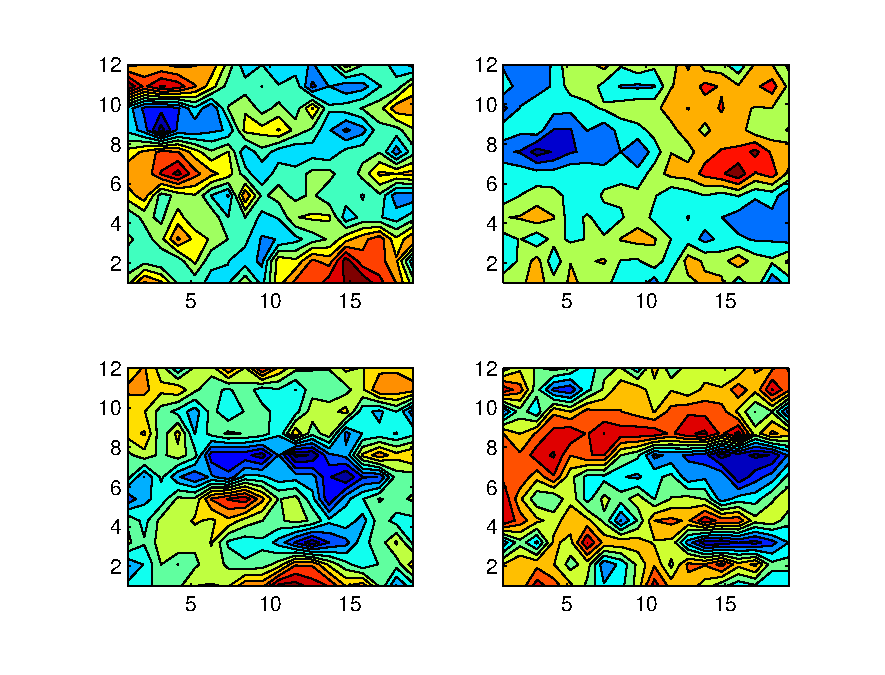
\includegraphics[width=0.5\textwidth]{aniso_data}
\caption{Four samples of anisotropic data}
\label{fig:aniso_data}}
\end{figure}


\subsection{Correlation Function for The Spatially Correlated Component}
The spatially correlatied component is modeled as random field with variance $\sigma^2$ and
correlation function $\rho(h)$ to be extracted.
Positive definiteness is the necessary condition for a parametric family of functions to define
a legitimate class of correlation functions. 
Note that the correlation function is an even function, i.e. $\rho(h) = \rho(-h)$, so that its Fourier transform is real. Moreover, because it is positive definite, based on the Bochner's theorem, its Fourier transform is positive. Some process may have further properties:
\begin{itemize}
\item
  monotonicity: correlations are monotonic decreasing against distance.
\item
  nonnegativeness: there is no negative correlaion.
\end{itemize}

\subsection{Correlation Function Considering Nugget Effect}
In the measurement data, apart from the spatially correlated component,
the purely random component and the unavoidable measurement error
also exist. Typically, the two components are modeled as random
variables with independent identical Gaussian distribution, or in short, Gaussian white noise.

When the two components are considered, the measurement data can still be regarded as a
Gaussian random field, but the correlation function will have a discontinuity at the origin.
This phenomenon is called ``nugget effect"~\cite{Diggle07}.

\section{Non-parametric Estimate}
\label{sc:lsq}
Given $N$ measurement samples $(y_1, y_2, \cdots, y_N) \in \domain{R}^n$. The measured covariance matrix $Y = = (1/N) \sum_{i=1}^N y_i y_i^{T}$. However, this matrix is unlikely to be positive definite. In~\cite{tbl}, the following minimization is suggested in order to obtain a nearest positive definite matrix $\Omega$:

\begin{equation}\label{eqn:lsq}
\begin{array}{cl}
\mbox{minimize} & ||\Omega - Y||_F \\
\mbox{subject to}& \Omega \succeq 0.
\end{array}
\end{equation}
where $||\dot||_F$ denotes the Frobenius norm and $A \succeq 0$ denotes the matrix $A$ is positive semidefinite. Note that the above problem is convex. In~[9], alternate projection method is used. The advantage of alternate projection method is that it is easy to implement. However, only linear convergence can be obtained. More importantly, the method is flexible enough for imposing other constriants. Fortunately, modern optimization techniques can solve the problem effectively and they are publicly available.

Similarly, the maximum likelihood estimation of covariance matrix is given by:
\begin{equation}\label{eqn:MLE}
\begin{array}{cl}
\mbox{minimize} & \log\det\Omega - \mathrm{Tr}(\Omega^{-1}Y) \\
\mbox{subject to}& \Omega \succeq 0.
\end{array}
\end{equation}
where $Tr(A)$ denotes the trace of $A$. Note that the first term is concave whereas second term is convex.
However, let $S = \Sigma^{-1}$, the function becomes convex in term of $S$

\begin{equation*}
  \begin{array}{cl}
	 \mbox{maximize}  & \log\det S - \mathrm{Tr}(S \cdot Y) \\
	 \mbox{subject to}& S \succeq 0, 
  \end{array}
\end{equation*}

However, very often we would like to add extra constraints directly to $\Omega$.We will discuss the $MLE$ estimation in more details in Section~\ref{sct:MLE}. Let us focus on the least squares estimation first.

If the process is known to be isotropic and the correlation model is known in prior, such as Mat\'{e}rn family. The covariance matrix $\Omega$ can further be expressed as a non-linear function of parameters, making the problem non-convex. It creates difficulties of numerical solving as mentioned in~\cite{tbl}.

In non-parametric approach, however, correlation functions are ��curved-fitted�� using linear combination of some basis functions:
\[
     \rho(h) = \sum_i p_i \Phi_i(h) 
\]
where $p_i$'s are the unknown coefficients to be fitted and $\Phi_i$'s are a family of basis functions. The corresponding covariance matrix $\Omega$ can be expressed as an affine function of the coefficients $p_1 F_1 + \cdots + p_m F_m$ where $\{F_k\}_{ij} = \Phi_k(s_j - s_i)$. Since it is an affine transformation, convexity is preserved.

Choice of $\Phi_i(h)$:
\begin{itemize}
\item
  $J_i(h)$: Bessel function, \\ 
            advantage: positive definite {\em if and only if} $p_i \ge 0$
		for all $i$. \\
            disadvantage: difficult to choose $i$, computational expensive.
\item
  $B_i(h)$: B-spline function, \\
            advantage: shapes are easier to control, \\
            e.g. monotonicity ($p_i \ge p_{i+1}$); \\
		disadvantage: not guarantee positive definite
\item
  $\cos((2\pi i/N)h)$: cosine functions
\end{itemize}
%% The comparison between the least squares estimation and maximum likelihood estimation is given in Fig.~\ref{fig:iso2d}
%% 
%% \begin{figure}[!tb]{\centering
%% 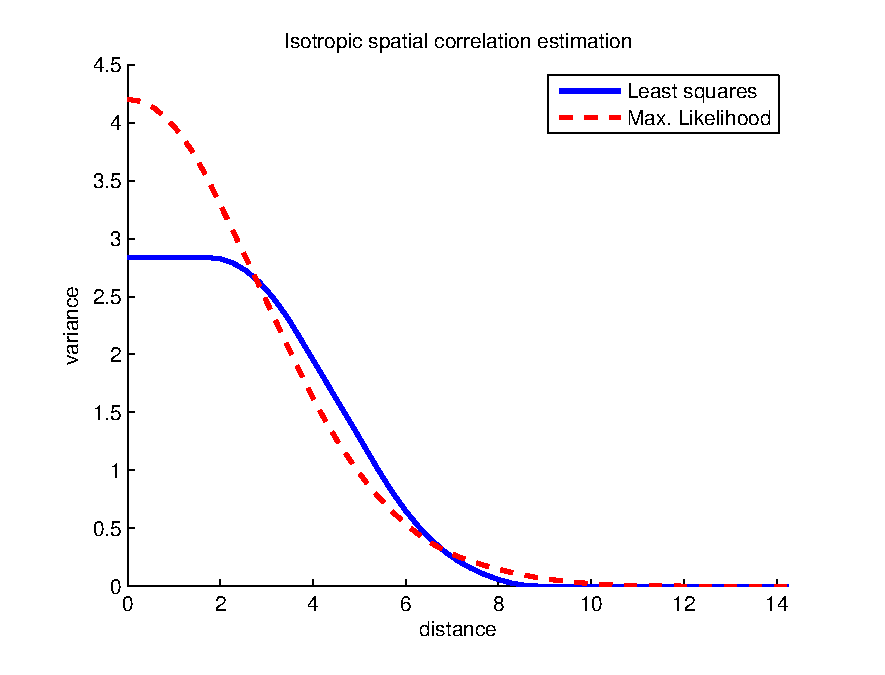
\includegraphics[width=0.4\textwidth]{iso2d}
%% \caption{Comparison between least squares and maximum likelihood estimation}
%% \label{fig:iso2d}}
%% \end{figure}

To ensure that the resulting function is positive definite, additional constraints can be imposed. Based on the Bochner's theorem, we may impose the fast Fourier transform to the discretized function, i.e., each element of
\[
   \mbox{real}(\mbox{FFT}(\{\Phi_i(x_k)\}) p
\]
is $\ge$ 0. Note that there is a trade-off of the granularity of discretization about the accuracy of the positive definiteness and efficiency.

\section{B-spline}
\label{sc:b-spline}
Let $\vectort = \{t_j\}_1^{n+k}$ be a nondecreasing sequence called
\emph{knot sequence}. The $j$th (normalized) 
\emph{B-spline} of order $k$ for $\vectort$ is denoted by $B_{j,k}$ and is
defined by  
\begin{equation}
B_{j,k}(x) = (t_{j+k}-t_j)[t_j,\ldots,t_{j+k}](t-x)_+^{k-1},\quad
\textrm{all } x \in R,
\end{equation}
which means that $B_{j,k}$ is the multiplication of $(t_{j+k}-t_j)$
and the $k$th divided difference of the truncated power function
$(t-x)_+^{k-1}$.

A spline function $f(x)$ of order $k$ with knot sequence $\vectort$ is any
linear combination of B-splines of order $k$ for the knot sequence
$\vectort$, i.e.,
\begin{equation}\label{eqn:spline_fn}
f(x)=\sum_{j=1}^n{p_{j} B_{j,k}(x)}.
\end{equation}

B-splines have the following fundamental properties~\cite{PGS}: 
\begin{itemize} \itemsep -0.5ex
\item Non-negative and local support: $B_{j,k}(x)$ is positive if
$x$ locates in $(t_j,t_{j+k})$ and is zero when $x$ is outside this
interval;  
\item Partition of unity: $\sum_{j=1}^n B_{j,k}(x)=1$ if
$x$ is in $[t_k,t_{n+1})$; 
\item Recurrence relation: $B_{j,k}(x)$ can be evaluated recursively
by $B_{j,k-1}(x)$ and $B_{j+1,k-1}(x)$. 
\item Convex hull: For $t_i<x<t_{i+1}$, the value of the spline
function $f(x)$ at the site $x$ is a strictly convex combination of
the $k$ numbers $p_{i+1-k},\ldots,p_i$.
\end{itemize}

This close relationship between the value of a spline and the
nearby B-spline coefficients provides the evidence that in order to
change part of $f$'s curve we only need to modify its nearby B-spline
coefficients. Because of this controllability, in CAGD the term
\emph{control point sequence} of the spline function 
$\sum_j{p_j B_{j,k}}$ with knot sequence $\vectort$ is defined as
$(t_{j,k}^*,p_j)_{j=1}^n$, where $t_{j,k}^*$ is sometimes called the
Greville site or the knot average,
\begin{equation}\label{eqn:aveknt}
t_{j,k}^*=\frac{t_{j+1}+\cdots+t_{j+k+1}}{k+1},\quad \forall j.
\end{equation}

For sake of simplicity, we use $t_j^*$ instead as long as the order
$k$ is fixed and no confusion is raised hereafter.

If the strictly increasing sequence $\vectorx = (x_i)_1^n$ of
data sites is given, then for a given function $g$, the spline function 
$f(x)$ defined in (\ref{eqn:spline_fn}) agrees with $g$ at $\vectorx$
if and only if  
\begin{equation}\label{eqn:B-interp}
\sum_{j=1}^n{p_j B_{j,k}(x_i)=g(x_i)},\quad i=1,\ldots,n.
\end{equation}
This is a linear system of $n$ equations in the vector 
$\vectorp=(p_j)_1^n$ of $n$ unknowns, with coefficient matrix 
$\big(B_{j,k}(x_i)\big)$, the \emph{spline collocation  matrix}. Hence
the matrix multiplication of~(\ref{eqn:B-interp})
can be written as $g(\vectorx) = \matrixB\cdot \vectorp$.

By solving out this system we obtain the B-spline
function $f(x)$. The advantage of using B-spline for interpolation or
approximation lies in the bandedness of
collocation matrix with bandwidth less than $k$. This is really a
consequence of B-spline's local support property. Another significant
property of the collocation matrix is total positivity, i.e., every
non-zero element of $\matrixB$ is positive. 

One of the advantages of using B-spline is that the monotonicity can be enforced by imposing a simple linear constraints on $p_i$, i.e. $p_{i+1} \ge p_{i}$. The nonnegativeness can be enforced by imposing constraints $p_i \ge 0$. Note however that it is not a neccessary condition so that it may overconstraint the result.

Fig.~\ref{fig:b-spline} shows results with different constraints of B-spline fitting.
\begin{figure}[!tb]{\centering
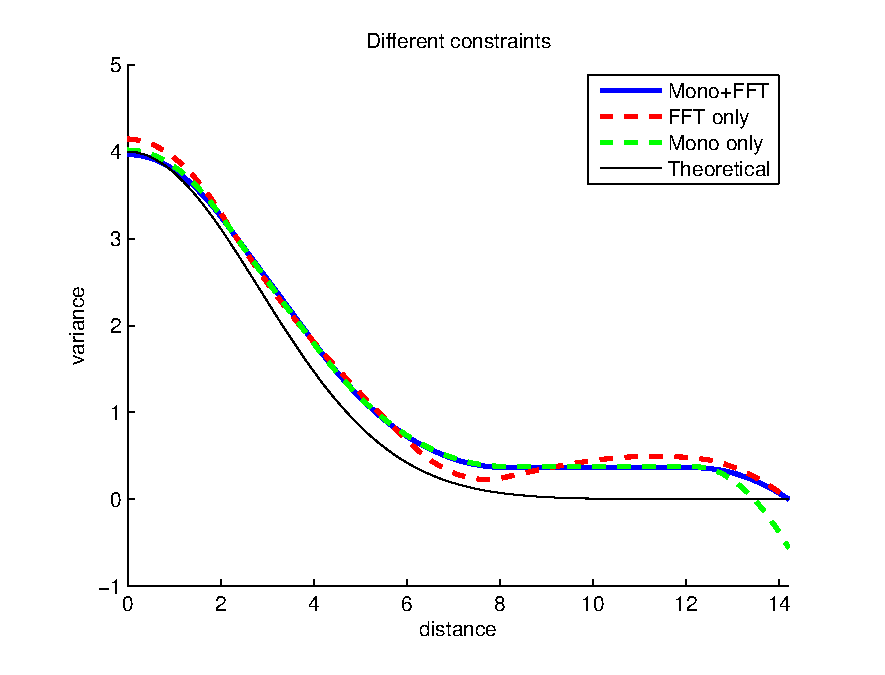
\includegraphics[width=0.4\textwidth]{b-spline}
\caption{B-spline fitting with different constraints}
\label{fig:b-spline}}
\end{figure}

\section{Non-Parametric Estimation for Anisotropic}
Result of anisotropic correlation function is in Fig.~\ref{exp2da}.

\begin{figure}[!tb]{\centering
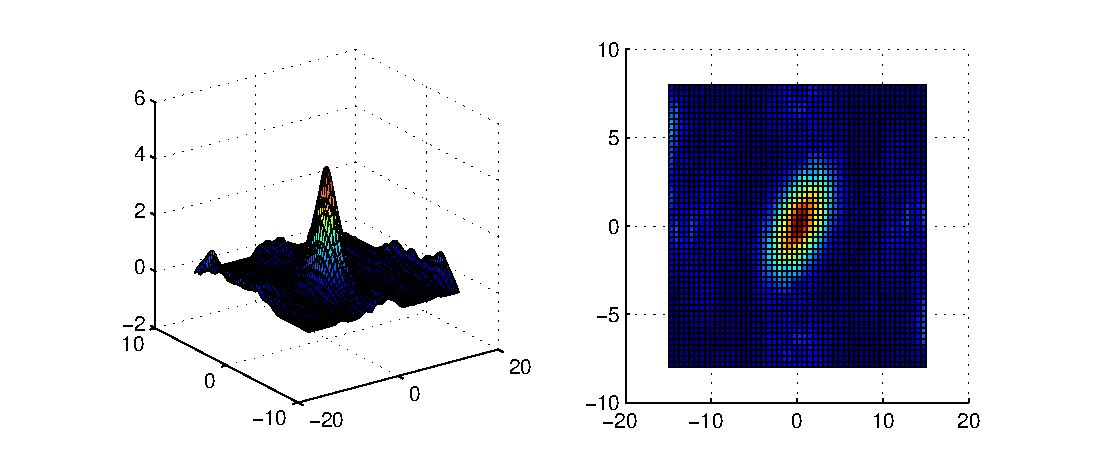
\includegraphics[width=0.5\textwidth]{exp2da}
\caption{Anisotropic model}
\label{fig:exp2da}}
\end{figure}



\section{Numerical Experiment}
\label{sc:experiment}
The proposed method was implemented in MATLAB on an Intel\textregistered~machine
with 3.0~GHz XEON\texttrademark~CPU.
Without real silicon measurement data, we synthesized a pseudo measurement process
and attained data from a batch of $M$ chips with $N$ sites on each chip.
The area of the chip is set to be 10mm$\times$10mm.

\section{Conclusions and Future Directions}
\label{sc:conclusions}

\section*{Acknowledgment}
The authors would like to thank...

% references section

% can use a bibliography generated by BibTeX as a .bbl file
% BibTeX documentation can be easily obtained at:
% http://www.ctan.org/tex-archive/biblio/bibtex/contrib/doc/
% The IEEEtran BibTeX style support page is at:
% http://www.michaelshell.org/tex/ieeetran/bibtex/
\bibliographystyle{IEEEtran}
% argument is your BibTeX string definitions and bibliography database(s)
\bibliography{Geostatistics,statistics,ref}% your bib database
%
% <OR> manually copy in the resultant .bbl file
% set second argument of \begin to the number of references
% (used to reserve space for the reference number labels box)
%% \begin{thebibliography}{1}
%% 
%% \bibitem{IEEEhowto:kopka}
%% H.~Kopka and P.~W. Daly, \emph{A Guide to \LaTeX}, 3rd~ed.\hskip 1em plus
%%   0.5em minus 0.4em\relax Harlow, England: Addison-Wesley, 1999.
%% 
%% \end{thebibliography}




% that's all folks
\end{document}


